% -*- TeX -*-

\documentclass{beamer}
\usepackage{amsmath}

\title{Crustal Deformation Modeling Tutorial}
\subtitle{Meshing with Complex Geometry}
\author{Charles Williams \\
  Brad Aagaard \\
  Matthew Knepley}
\institute{
\includegraphics[scale=0.4]{../../logos/cig_blackfg}}
\date{June 26, 2017}


% ---------------------------------------------------- CUSTOMIZATION
\renewcommand{\thispdfpagelabel}[1]{}
\newcommand{\important}[1]{{\color{red}#1}}
\usetheme{CIG}

% --------------------------------------------------------- DOCUMENT
\begin{document}

% ------------------------------------------------------------ SLIDE
\maketitle

% ========================================================== SECTION
\section{Meshing}
\subsection{General steps}

% ------------------------------------------------------------- LOGO
\logo{
\includegraphics[height=4.5ex]{../../logos/cig_blackfg}}

% ------------------------------------------------------------ SLIDE
\begin{frame}
  \frametitle{Meshing Complex Geometry}
  \summary{Steps in creating a mesh}
  
  \begin{itemize}
  \item Determine geometric features needed
    \begin{itemize}
    \item Fault geometry
    \item Topography
    \item Sharp structural boundaries
    \item Magma sources with complex geometry
    \end{itemize}
  \item Create spline curve (2D) or NURBS surface (3D) in CUBIT/Trelis
  \item If using surface in several models export it for future use
  \item Use surfaces within CUBIT/Trelis to webcut volumes
  \item Choose discretization according to type of problem
  \end{itemize}

\end{frame}

% ========================================================== SECTION
\subsection{Subduction meshing Example}

% ------------------------------------------------------------ SLIDE
\begin{frame}
  \frametitle{Meshing of a subduction zone}
  \summary{3-D coarse meshing of Cascadia with a simulated splay fault}
  
  \begin{itemize}
  \item Three-dimensional Cascadia subduction zone example\\
    \important{{\tt examples/3d/subduction/mesh}}
    \begin{itemize}
    \item Generate fault surfaces and export as ACIS files using
      \important{\tt generate\_surfjou.py} script to create
      \important{\tt geometry\_surfs.jou} file.
      \begin{itemize}
      \item Generate subduction interface from SLAB1.0 contours --
        script performs georeferencing to our local coordinates system
        as well as creating journal files.
      \item Generate slab bottom as an offset from subduction interface.
      \item Generate fictitious splay fault along a contour of subduction
        interface.
      \end{itemize}
    \item Generate volume geometry using \important{\tt geometry.jou}.
    \item Generate mesh using either \important{\tt mesh\_hex.jou} or
      \important{\tt mesh\_tet.jou}.
    \end{itemize}
  \end{itemize}


\end{frame}


% ========================================================== SECTION
\subsection{Problem geometry}

% ------------------------------------------------------------ SLIDE
\begin{frame}
  \frametitle{Simulated Cascadia Subduction Zone}
  \summary{Geometry with subduction thrust, slab and crust bottom, and
    splay fault}
 
  \vfill
  \begin{center}
    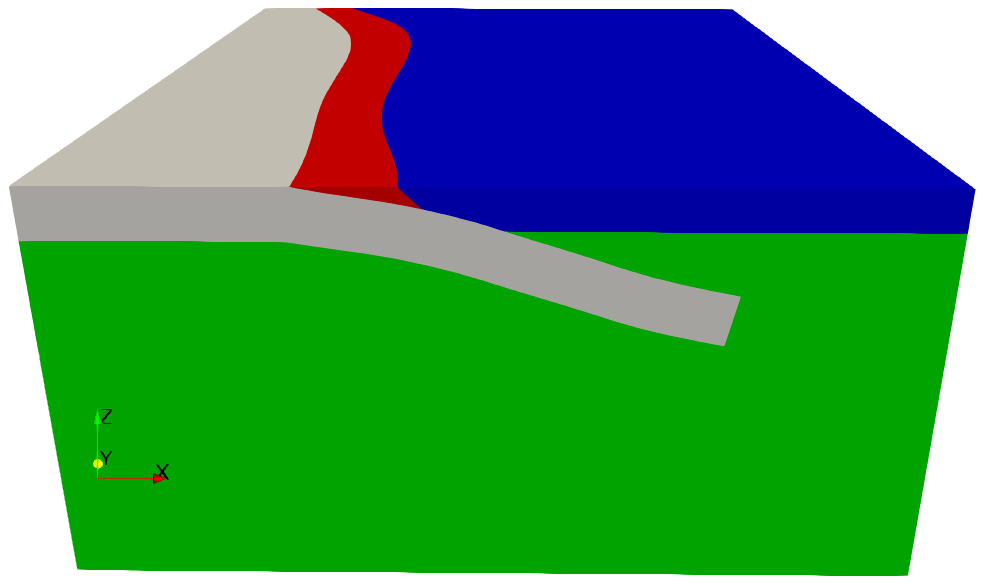
\includegraphics[height=6.1cm]{figs/subduction3d_conceptualmodel}
  \end{center}
  \vfill

\end{frame}


% ========================================================== SECTION
\subsection{Tetrahedral mesh}

% ------------------------------------------------------------ SLIDE
\begin{frame}
  \frametitle{Tetrahedral mesh generated for Cascadia problem}
  \summary{Constant resolution mesh with approximately 144k cells}
 
  \vfill
  \begin{center}
    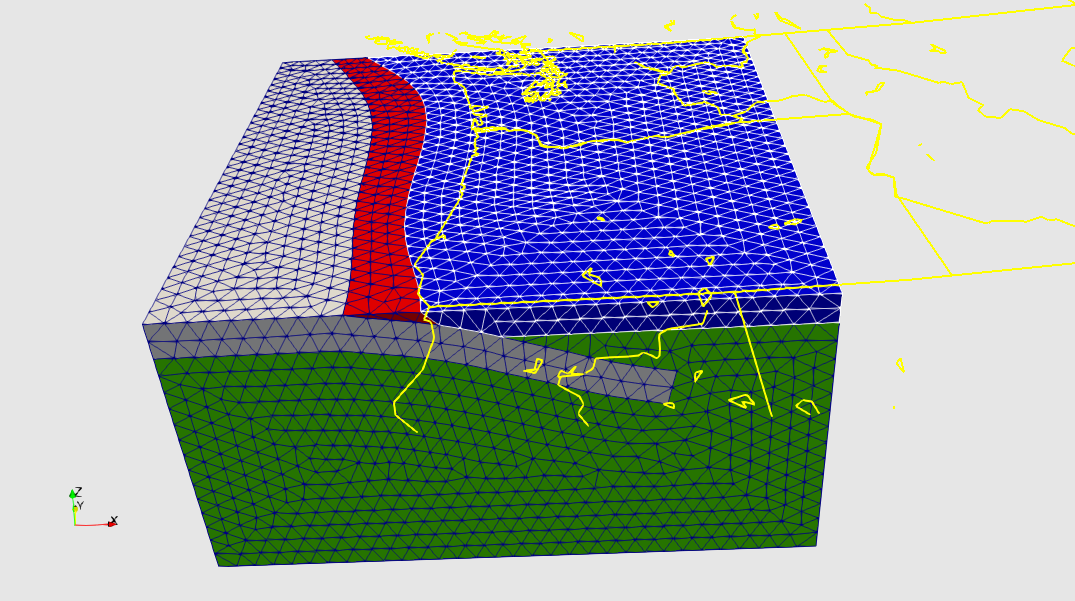
\includegraphics[height=6.1cm]{figs/subduction3d_tetmesh}
  \end{center}
  \vfill
 
\end{frame}


% ------------------------------------------------------------ SLIDE
\subsection{What's missing}

\begin{frame}
  \frametitle{What's missing}
  \summary{Additional modifications for real problems}
  
  \begin{itemize}
  \item Mesh needs to be larger to move boundaries away from region of
    interest.
    \begin{itemize}
    \item Enclose inner region in a larger box.
    \item Let Trelis/Cubit mesh internal surfaces (untested).
    \end{itemize}
  \item The mesh is much too coarse and not graded.
    \begin{itemize}
    \item Use sizing function to create a nicely graded mesh. See
      \important{\tt examples/meshing/cubit\_cellsize} for an example.
    \end{itemize}
  \end{itemize}

\vfill
NOTE:  If anyone does not have Cubit/Trelis, the mesh is available on the
PyLith wiki:
\important{https://wiki.geodynamics.org/software:pylith:cdm2017}
 
\end{frame}



% ======================================================================
\end{document}


% End of file
